% !TeX root = ../main.tex
% Appendix: the ablation mirrors the main text defers (DeepSeek-8B, TraceElephant,
% and the validation-selected transfer grids). Created 2026-08-24. Numbers are
% typed from the `--print-tables` dump of scripts/ablations/plot_figures.py, which
% reads results-ablations/*.tsv; the headline cells also appear in
% experiments/todo.md. Figures: artifacts/ablations/ -> assets/.

\section{Additional ablation results}
\label{app:deepseek-ablations}

The main text ablates \soap on WW-AG and WW-HC with backbone Qwen3.5-9B (Section~\ref{sec:exp:analysis}). This appendix repeats every ablation on the remaining cells --- TE-Cap and TE-Mag on Qwen3.5-9B, and all four subsets on DeepSeek-8B --- under the same protocol: start from the selected configuration of Table~\ref{tab:main}, vary one axis, hold everything else fixed. One caveat recurs: DeepSeek-8B's selected configuration on WW-HC has $\gamma{=}0$, so rescoring is a no-op there and every row or bar that varies only the rescoring equals the base score by construction.

\subsection{Scoring functions}

Table~\ref{tab:scorefn-app} extends Table~\ref{tab:scorefn} to the remaining cells. The spectral band wins or ties every column. Where the selected band starts at component $0$ (WW-HC, TE-Cap, TE-Mag on both backbones) the top subspace \emph{is} the selected band, so those ties hold by construction; the discriminating column is WW-AG, where the selected band starts at component $1$ and dropping the leading direction is worth 24--26 points over the top subspace on both backbones. DeepSeek-8B's near-tie between the full spectrum and the band on TE-Cap (39.53 vs.\ 40.31) follows from its wide selected band $[0, 18)$, which nearly spans the computed spectrum.

\begin{table}[h]
\centering
\small
\setlength{\tabcolsep}{5pt}
\caption{\textbf{Alternative per-step scoring functions, remaining cells.} Step-level accuracy (\%) with no rescoring; orientations fixed as in Table~\ref{tab:scorefn}. Best per column in \best{bold}.}
\label{tab:scorefn-app}
% results-ablations/a1_scorefn/scorefn.tsv (A1).
\begin{tabular}{l cc cccc}
\toprule
 & \multicolumn{2}{c}{Qwen3.5-9B} & \multicolumn{4}{c}{DeepSeek-8B} \\
\cmidrule(lr){2-3}\cmidrule(lr){4-7}
Scoring function & TE-Cap & TE-Mag & WW-AG & WW-HC & TE-Cap & TE-Mag \\
\midrule
Perplexity           & 6.20  & 7.97  & 4.23  & 14.94 & 5.43  & 3.62 \\
Random subspace      & 17.83 & 7.25  & 10.58 & 16.09 & 12.40 & 12.32 \\
Top subspace         & \best{33.33} & \best{21.01} & 14.29 & \best{28.74} & \best{40.31} & \best{29.71} \\
Tail subspace        & 6.20  & 1.45  & 10.58 & 4.60  & 18.60 & 5.07 \\
Full spectrum        & 32.56 & 17.39 & 16.93 & 19.54 & 39.53 & 22.46 \\
Norm $\ell_1$        & 15.50 & 5.07  & 33.86 & 16.09 & 20.16 & 8.70 \\
Norm $\ell_2$        & 27.13 & 15.22 & 15.87 & 20.69 & 26.36 & 9.42 \\
\rowcolor{Gray}
Spectral band (ours) & \best{33.33} & \best{21.01} & \best{38.62} & \best{28.74} & \best{40.31} & \best{29.71} \\
\bottomrule
\end{tabular}
\end{table}

\subsection{Rescoring designs}

Table~\ref{tab:weights-app} is the DeepSeek-8B counterpart of Table~\ref{tab:weights}. The picture repeats: the unnormalized sum collapses toward predicting the first step, the normalized mean hovers around the base score, and no position heuristic reaches attention-guided rescoring where rescoring matters (WW-AG, TE-Cap, TE-Mag). The WW-HC column is flat at the base score because that cell selected $\gamma{=}0$; the same holds for six of the seven CE subsets on DeepSeek-8B, which is why the CE column moves little.

\begin{table}[h]
\centering
\small
\setlength{\tabcolsep}{5pt}
\caption{\textbf{Alternatives to attention-guided rescoring, DeepSeek-8B.} Step-level accuracy (\%) on all five subsets; rows as in Table~\ref{tab:weights}. Best per column in \best{bold}.}
\label{tab:weights-app}
% results-ablations/a2_weights.tsv (with_gt=False) + a3_position.tsv (selected rows;
% CE macro-averaged over its seven subsets). Selected lambdas, z-scored / raw:
% WW-AG 0.1 / 1.0, WW-HC 0.1 / 1.0, TE-Cap 0.4 / 1.0, TE-Mag 0.4 / 0.1.
\begin{tabular}{l ccccc}
\toprule
Rescoring design & WW-AG & WW-HC & CE & TE-Cap & TE-Mag \\
\midrule
Base score (no rescoring)   & 38.62 & \best{28.74} & 64.19 & 40.31 & 29.71 \\
\addlinespace[2pt]
\multicolumn{6}{@{}l}{\textit{Content-agnostic dependency weights}} \\
\quad Uniform (unnormalized) & 16.40 & \best{28.74} & 57.01 & 10.08 & 4.35 \\
\quad Uniform (normalized)   & 35.45 & \best{28.74} & 62.14 & 41.86 & 28.99 \\
\addlinespace[2pt]
\multicolumn{6}{@{}l}{\textit{Position heuristics}} \\
\quad Temporal bias, z-scored & 38.10 & \best{28.74} & 63.33 & 41.09 & 28.26 \\
\quad Temporal bias, raw      & 38.62 & 3.45  & 42.05 & 6.20  & 20.29 \\
\quad Earliest of top-$5$     & 29.10 & 10.34 & 2.39  & 13.18 & 5.80 \\
\addlinespace[2pt]
\rowcolor{Gray}
Attention-guided (ours)     & \best{45.50} & \best{28.74} & \best{64.68} & \best{42.64} & \best{30.43} \\
\bottomrule
\end{tabular}
\end{table}

\subsection{Context window of the dependency weights}

Table~\ref{tab:attnsel} varies how many predecessors each step's attention distributes blame over, $w \in \{1,2,3,4,5,\text{all}\}$, with everything else at the selected configuration. The preference is dataset-shaped. On Who\&When both backbones favor the sharpest window: accuracy is highest at $w{=}1$--$2$ and declines toward all predecessors (47.62 at $w{=}1$ vs.\ 40.21 at all, Qwen3.5-9B WW-AG) --- restricting each step to its few strongest dependencies keeps the correction targeted, while averaging over every predecessor dilutes it back toward the uniform weights of Table~\ref{tab:weights}. On TE-Cap wider windows win on both backbones, up to all predecessors on DeepSeek-8B. A badly chosen $w$ can land below the base score (Qwen3.5-9B TE-Mag at $w{=}1$: 15.94 vs.\ 21.01), so $w$ is selected, not fixed.

\begin{table}[h]
\centering
\small
\setlength{\tabcolsep}{5pt}
\caption{\textbf{Context window $w$ of the dependency weights.} Step-level accuracy (\%) for $w$ strongest predecessors per step, everything else at the selected configuration; the selected $w$ in \best{bold}. DeepSeek-8B's selected $\gamma$ on WW-HC is $0$, so that row is constant by construction.}
\label{tab:attnsel}
% results-ablations/a4_window.tsv (A4, pure grid filter); moved here from the main
% text 2026-08-24 (the main-text table covered WW only).
\begin{tabular}{ll cccccc}
\toprule
Backbone & Subset & $w{=}1$ & $2$ & $3$ & $4$ & $5$ & all \\
\midrule
\multirow{4}{*}{Qwen3.5-9B}
 & WW-AG  & \best{47.62} & 41.80 & 40.74 & 40.21 & 40.21 & 40.21 \\
 & WW-HC  & 33.33 & \best{34.48} & 32.18 & 32.18 & 32.18 & 32.18 \\
 & TE-Cap & 28.68 & 29.46 & 34.88 & 34.88 & \best{35.66} & 34.88 \\
 & TE-Mag & 15.94 & 20.29 & 18.84 & \best{23.19} & 18.84 & 18.12 \\
\midrule
\multirow{4}{*}{DeepSeek-8B}
 & WW-AG  & \best{45.50} & 38.62 & 33.33 & 34.39 & 37.57 & 37.57 \\
 & WW-HC  & 28.74 & 28.74 & 28.74 & 28.74 & 28.74 & \best{28.74} \\
 & TE-Cap & 35.66 & 38.76 & 41.09 & 41.09 & 41.86 & \best{42.64} \\
 & TE-Mag & \best{30.43} & 30.43 & 30.43 & 29.71 & 28.99 & 28.99 \\
\bottomrule
\end{tabular}
\end{table}

\subsection{Sensitivity to the hyperparameters}

Figure~\ref{fig:sensitivity-app} repeats Figure~\ref{fig:sensitivity} on all eight (backbone, subset) cells and adds the window $w$ of Table~\ref{tab:attnsel} as a panel. Two regularities hold across backbones. First, $\gamma$ has the same two regimes: WW-AG climbs toward large $\gamma$ on DeepSeek-8B as on Qwen3.5-9B, while every other cell peaks at $\gamma \in \{0.1, 0.2\}$ and decays beyond. Second, the selected layer is the per-layer optimum of post-rescoring accuracy in seven of the eight cells (the exception is DeepSeek-8B TE-Mag, where layer 9 edges the selected layer 10 by 1.4 points); WW-HC concentrates in the last layer on both backbones, and DeepSeek-8B consistently prefers the late attention band (24--32).

\begin{figure}[h]
\centering
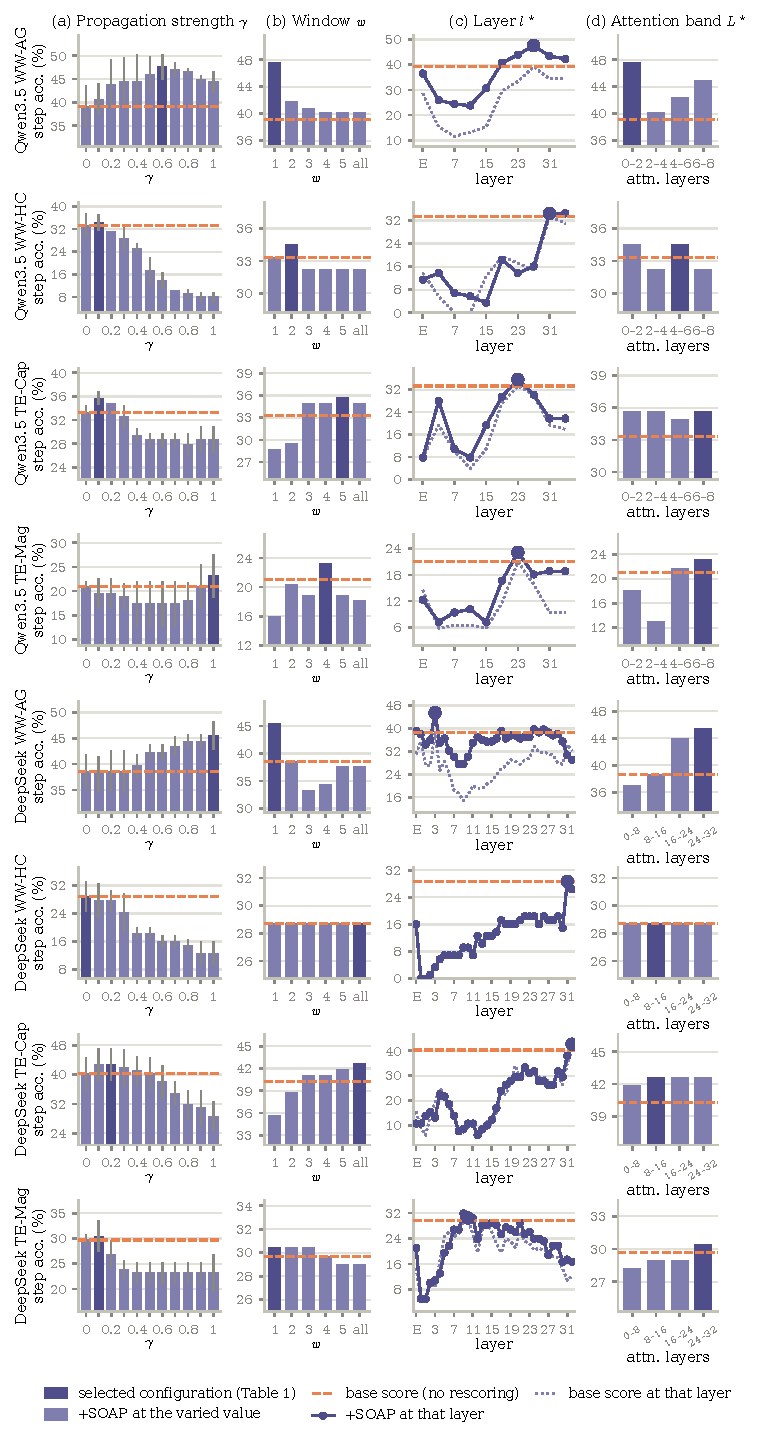
\includegraphics[width=\textwidth]{assets/fig_sensitivity_appendix.pdf}
\caption{\textbf{Sensitivity of \soap, all cells.} As Figure~\ref{fig:sensitivity}, for all four subsets on both backbones, with the context window $w$ added as panel (b): (a) propagation strength $\gamma$, (b) window $w$, (c) representation layer $l^\star$ (solid: after rescoring; dotted: base score at that layer; large marker: selected layer; DeepSeek-8B sweeps every block, Qwen3.5-9B every fourth), (d) attention band $L^\star$. The dashed orange line is the base score of the selected configuration (no rescoring). DeepSeek-8B on WW-HC selected $\gamma{=}0$, so its $w$ and attention-band panels are flat by construction.}
\label{fig:sensitivity-app}
\end{figure}

\subsection{Cross-distribution transfer and reference-data quantity}

Figure~\ref{fig:transfer-app} gives all four transfer grids: both backbones under the optimistic \emph{test-selected} convention of Table~\ref{tab:main} (the configuration for each source--target pair is chosen on the target's test split, exactly as the in-distribution numbers are) and under the \emph{validation-selected} convention (chosen on the target's validation split, which for the cross setting pools the target's train and validation files, since the target's train split is not used for fitting). The diagonal of every grid is the in-distribution number of Table~\ref{tab:main}. Under the test convention most cross cells land within a few points of the diagonal, and a foreign reference can even match or beat the in-distribution one on DeepSeek-8B (WW-HC$\to$TE-Cap ties 42.64; WW-HC$\to$TE-Mag reaches 33.33 vs.\ 30.43). The validation convention restores the gap --- the diagonal wins every column on both backbones --- but the degradation is graded, not catastrophic (DeepSeek-8B WW-HC$\to$WW-AG keeps 39.68 of 45.50). Freezing the source's whole configuration instead of re-selecting collapses transfer (Qwen3.5-9B WW-AG$\to$WW-HC: 3.45), so what is distribution-specific is chiefly the hyperparameter configuration, not the spectral reference.

\begin{figure}[h]
\centering
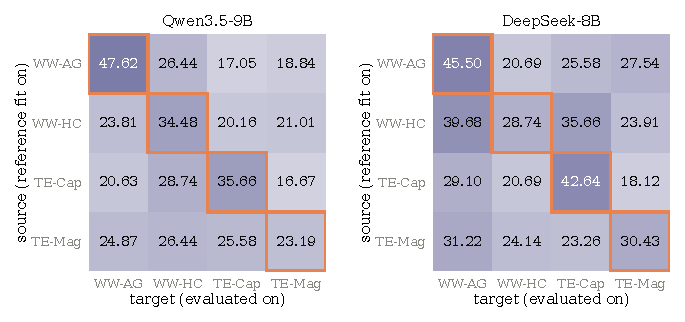
\includegraphics[width=0.9\textwidth]{assets/fig_transfer_appendix.pdf}
\caption{\textbf{Cross-distribution transfer, all grids.} Step-level accuracy (\%) of \soap with the reference fitted on the source subset (rows) and the configuration re-selected and evaluated on the target subset (columns), for both backbones, under the test-selected (top) and validation-selected (bottom) conventions. The outlined diagonal is the in-distribution number of Table~\ref{tab:main} in every grid.}
\label{fig:transfer-app}
% results-ablations/e1_transfer.tsv (row=soap); the frozen-anchor design is in
% e1_transfer_frozen-anchor.tsv.
\end{figure}

Table~\ref{tab:datasize-app} completes Figure~\ref{fig:transfer}(b). With a third of the reference corpus (6--12 trajectories) every cell is within about four points of its full-data accuracy, and most within one or two. Because the configuration is re-selected at each fraction on the test split, a small fit can occasionally score above the full one (DeepSeek-8B WW-HC and TE-Mag at $10\%$); this is selection noise on tiny fits, not a real gain.

\begin{table}[h]
\centering
\small
\setlength{\tabcolsep}{4pt}
\caption{\textbf{Quantity of unlabeled reference data, all cells.} Step-level accuracy (\%) before ($S$) and after ($+\soap$) rescoring when the reference is fit on $\{10, 20, 30\}\%$ of the corpus, validation and test fixed, full configuration re-selected per fraction.}
\label{tab:datasize-app}
% results-ablations/a7_datasize.tsv (A7); n_train per seed: WW-AG 12/25/37,
% WW-HC 6/11/17, TE-Cap 8/17/25, TE-Mag 9/18/27.
\begin{tabular}{l cc cc cc cc}
\toprule
 & \multicolumn{2}{c}{WW-AG} & \multicolumn{2}{c}{WW-HC} & \multicolumn{2}{c}{TE-Cap} & \multicolumn{2}{c}{TE-Mag} \\
\cmidrule(lr){2-3}\cmidrule(lr){4-5}\cmidrule(lr){6-7}\cmidrule(lr){8-9}
Reference data & $S$ & $+\soap$ & $S$ & $+\soap$ & $S$ & $+\soap$ & $S$ & $+\soap$ \\
\midrule
\multicolumn{9}{@{}l}{\textit{Qwen3.5-9B}} \\
\quad 10\% & 35.98 & 43.39 & 33.33 & 33.33 & 33.33 & 34.88 & 21.74 & 23.19 \\
\quad 20\% & 38.10 & 44.44 & 33.33 & 33.33 & 33.33 & 34.88 & 21.74 & 23.19 \\
\quad 30\% & 39.15 & 47.62 & 33.33 & 34.48 & 33.33 & 35.66 & 21.01 & 23.19 \\
\addlinespace[2pt]
\multicolumn{9}{@{}l}{\textit{DeepSeek-8B}} \\
\quad 10\% & 36.51 & 37.04 & 27.59 & 29.89 & 37.21 & 41.86 & 31.16 & 31.88 \\
\quad 20\% & 38.62 & 46.03 & 28.74 & 28.74 & 39.53 & 42.64 & 30.43 & 30.43 \\
\quad 30\% & 38.62 & 45.50 & 28.74 & 28.74 & 40.31 & 42.64 & 29.71 & 30.43 \\
\bottomrule
\end{tabular}
\end{table}
